%!TEX root = ../../thesis.tex

\section{Discussion}
\label{sec:chisquared_discussion}




\section{Discussion}
\label{sec:discussion}
The spectral differential and the synthetic recovery methods attempted here were both unsuccessful in a detection of the {BD} companion spectra.
The upper mass limits of \(600^{+20}_{-40}\) we set for these companions is very high, roughly six times higher then the {BD} mass limit \(\sim 80-90\)\Mjup{}.
We discuss potential reasons and solutions for these poor results below, list the lessons learned in this exploratory study, and provide some guidance for any future attempts with these methods.


\subsection{Synthetic recovery limitations}
\label{subsec:limitations}
In this section we discuss some of the limitations from this synthetic recovery method and some options to overcome some of these.

\subsubsection{Mismatch in synthetic models}
\label{subsubsec:mismatch}
We believe the mismatch between the observation and synthetic spectra is the main cause of the unsuccessful companion detection, impacting the recovery in two ways.
The mismatch causes the \textchisquared{} values to be large in general, but also causes the companion temperature to be pushed to higher temperatures.

In our examples the \logg{} and metallicity of the synthetic models are held fixed, leaving only temperature to vary.
The temperature impacts the synthetic spectral models in two main ways: the flux level of the continuum; and the number and strength of the absorption lines.
In the binary model the contributions from the individual components is scaled by the flux ratio.If the temperature of the companion increases then the flux and radius of the companion increases.
Its contribution of the companion to the binary model increases and the flux ratio \FoneFtwo{} decreases.
This effectively makes the lines of the spectrum of the host component relatively smaller in the normalized binary model spectrum.
Due to the initial mismatch of synthetic spectral lines, a decrease in relative strength of the host lines decreases the \textchisquared{} value, and is a better "match" to the observation.
This causes the recovered temperature of the companion to be higher than expected, >2000\K{} higher if allowed by the exploration grid.
The \textchisquared{} approach is dominated by reducing the mismatch in the spectrum of the host rather than detecting the spectra of the companion.
This spectral mismatch is not observed in the simulations in \cref{subsec:simulated_binaries} since they are created using the synthetic spectra themselves, and hence they do recover the correct host spectra.


\subsubsection{Line contribution of faint companions}
\label{subsubsec:line_contributions}
We calculate the line depths of the synthetic companion spectra to determine the \snr{} levels required to detect the lines of the binary companions.
One thing easy to overlook when attempting to detect the binary companion at low flux ratios is the actual contribution of the spectral lines of the companion.
The flux ratio of the continuum for our most promising target is \FtwoFone{}\(\sim\)3\% with the other targets having an expected flux ratio around 1\%, and some well below.
The spectral lines of the individual components which are the features we are trying to detect with the binary model, have depths on average around 10--20\% of their respective continua,  at-least between 2110--2160\nm{}.
In effect, the companion line features have a depth \(\ll 1\%\) relative to the continuum of the combined spectra.

In \cref{tab:line_contributions} we calculate some properties of the spectral lines in the {PHOENIX-ACES} library between 2110--2160\nm{}.
We count the number of spectral lines (\emph{no. lines}) deeper than 5\%, and take the average depth (\emph{avg. depth}) of these lines.
The contribution \emph{cont. depth} of the companion lines to a combined spectrum accounts for the flux ratio between the two components.
Here we use a Sun-like host with \(\teffsub{1}\)=5800\K{}.
This simplified combination neglects the continuum shapes of both spectral components and uses the average flux ratios for this wavelength range.
The {PHOENIX-ACES} spectra in the temperature range of 2500--5000\K{} shown in \cref{fig:comp_spectra} can be used to get a visual indication of the line density and depth measured here.

There are more lines >5\% deep for the lower temperature spectra, with 360--460 lines in this wavelength range, to be compared with the 31 deep absorption lines found in a Sun-like spectrum.
The average line depth of these lines is also larger than the Sun-like spectrum, around twice as deep.
However, when combined, the contribution of the companion lines is 1--2 orders of magnitude smaller than the hosts lines due to the low continuum flux ratios.

For example, with the synthetic model for the companion of {HD~211847}, the average contributions of lines >5\% become only 0.3\% deep in a binary with the Sun-like spectrum.
For a companion with a temperature of 2300\K{} (the lower {PHOENIX-ACES} temperature limit) the deepest lines contribute lines around 0.1\%.

%{\bl We use the contributed line depth values to calculate the \snr{} level required to have Gaussian noise of the same height and the observed \snr{} required to achieve equivalent contribution from all N lines of the spectrum, \(\rm \textrm{SNR}_N = \textrm{SNR} /\sqrt{N}\).
%This is for the synthetic spectra which have many more lines than the observed spectra in this wavelength range.}

The \snr{} of the observed spectra is between 100--300, which is below the \snr{} of 323 needed for the detection of the low-mass star companion of {HD~211847} with temperature of 3200\K{} and \logg{} 5.0.
For our other targets with {BD} companions at and below the {PHOENIX-ACES} temperature range, we would need observed \snr{} >800 to detect the individual spectral lines of the companion.
With the \snr{} increasing with \(\sqrt{N}\) this would require the observational time for each target to be increased by a factor of \(\sim\)~10--64.

Our non-detection of binary companions with low flux ratios is consistent with other works.
For example~\citet{nemravova_xtauri_2016} performed extensive spectral analysis of a quadruple-star system \object{$\xi$ Tauri} using 227 spectra in 3 different wavelength bands with \(R=10\,000--48\,000\).
Of the four stars in the system they were unable to detect the spectral component of the star which had a luminosity ratio below 1\%.
%!TEX root = ../nir_companions.tex

\begin{table}
    \small
    \centering
    \begin{threeparttable}[b]
        \caption[Analysis of spectral line depths.]{Contribution of synthetic lines within 2\,110--2\,160\nm{} of synthetic {PHOENIX-ACES} spectra to a binary model. \(F_{2}/F_{1}\) is the continuum flux ratio between a spectrum with the given \Teff{} and \logg{} and a Sun-like spectrum with \(\teff{}=5\,800\),\logg{} = 4.5 (right most column). \emph{No.\ lines} is the number of spectral lines deeper than 5\% from the continuum of the individual spectra while \emph{avg.\ depth} is the mean depth of those lines. \emph{Cont.\ depth} is the average contribution, or depth, of these lines in the combined spectrum of a binary with a Sun-like spectrum. The \snr{} is signal-to-noise level required to have Gaussian noise \(\sigma=1/\snr{}\)  equal to the \emph{cont.\ depth} level in the binary model. All synthetic spectra used here have \feh{}=0.0.}
        \begin{tabular}{*7c}
            \toprule
            \teff{} (K)  & \multicolumn{2}{c}{2300} & \multicolumn{2}{c}{3200} & 5\,800 (\(\rm F_1\))\\
           \logg{} & 5.0 & 4.5  & 5.0 & 4.5 & 4.5 \\
            \midrule
            \(F_2/F_1\) & 0.006 & 0.019 & 0.029  & 0.091 & 1.000 \\
            % {>2\%}  & no. lines & 470 &  463 & 414  & 444 & 111 \\
            % & avg.\ depth & 0.20 & 0.23 & 0.10  & 0.12 & 0.04 \\
            % & cont. depth \tablefootmark{a} & 0.0012 &  0.0043 & 0.0028 &  0.0100 &  0.0333\tablefootmark{b} \\
            % \midrule
            no.\ lines & 464 & 463 & 365  & 413 & 31 \\
            avg.\ depth & 0.2  & 0.23 & 0.11 & 0.12 & 0.10 \\
            cont.\ depth\tnote{a} &  0.0012 & 0.0043 &  0.0031 & 0.0100 &  0.0833\tnote{b} \\
            \snr{}  & 833 & 232 & 323  & 100 & 12 \\
            %  {SNR}\(\rm _N\)  & 39 & 11 & 17  & 5 & 2 \\
            \bottomrule
        \end{tabular}\label{tab:line_contributions}
        \begin{tablenotes}
            \item [a] avg.\ depth \(\times~ \rm F_2 / (F_1 + F_2)\), where \(F_1\) is the component in the far right column.
            \item[b] avg.\ depth \(\times~ \rm F_1 / (F_1 + F_2)\), where \(\rm F_2\) is for the companion with \teff{}=3200, \logg{}=4.5.
        \end{tablenotes}
    \end{threeparttable}
\end{table}



\begin{figure}
    \centering
    %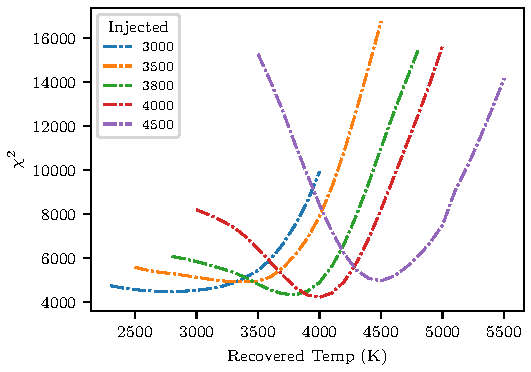
\includegraphics[width=0.7\linewidth]{figures/companion_recovery/chi2_shape_investigation}
    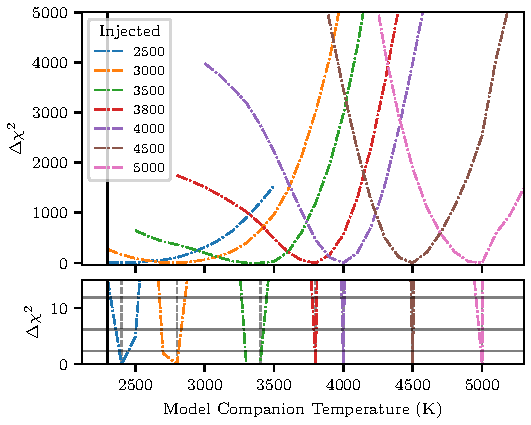
\includegraphics[width=0.7\linewidth]{figures/companion_recovery/chi2_shape_investigation_with_delta}
    \caption[Shape of simulated \textchisquared{} with different injected companion temperatures.]{Top: Companion temperature verses \textchisquared{} for simulations with different injected companion temperatures.
        The other fixed parameters for these fully synthetic simulations was \(\teffsub{1}=5200\)\K{}, \(\logg_{1}=4.5\), \(\logg{}_{2}=5.0\), and both \feh{}=0.0.
        A fixed Gaussian noise corresponding to a \snr{} of 300 was used.
        Bottom: A close up view of \textchisquared{} below 15.
        The three horizontal grey lines indicate the 1-, 2-, 3-$\sigma$ with 2 degrees of freedom.
        The vertical dotted lines indicate the location of the minimum \textchisquared{} recovered for each companion.
        The black solid vertical in both panels shows the 2300\K{} cut-off of the {PHOENIX-ACES} models}
    \label{fig:injection_shape}
    %\label{fig:chi2shapeinvestigation}
\end{figure}

\todo{}
\subsubsection{\(\chi^2\) asymmetry} 
\label{subsubsec:chi2_assymetry}

To try and understand this recovered companions further investigation into the \textchisquared{} space was performed of the {HD30501} synthetic simulation.
The minimum \textchisquared{} contours achieved for each companion temperature in the grid, regardless of \Rvtwo{} are shown in \cref{fig:injection_shape}.
This is done for seven different injected companion temperatures, \(\teffsub{2}\), between 2500 and 4500\K{}.
For the higher temperature companions, the \textchisquared{} is parabolic in shape, recovering the correct temperature, as expected.
At lower temperatures there is a strong asymmetry in the \textchisquared{} with it flattening out on the lower temperature side.
The 1-, 2-, 3-\(\sigma\) values (with 2 degrees of freedom) of 2, 6 and 11 above the minimum \textchisquared{} are not shown in the bottom panel of \cref{fig:injection_shape} which is a close-up around the minimum \textchisquared{} as they are indistinguishable in the top panel due to the extreme \textchisquared{} y-scale.
The black vertical line indicates the 2300\K{} temperature limit of the {PHOENIX-ACES} models.

In \cref{fig:injection_shape} we showed that the shape of the recovered \textchisquared{} becomes asymmetric when dealing with companion temperatures below around 3800\K{}.
A visual inspection of the spectra reveals the likely cause.
In \cref{fig:comp_spectra} we show the corresponding spectra between 2111--2165\nm{}.
As the temperature decreases the strongest lines become less prominent, disappearing progressively among the other many small lines that appear at lower temperatures.
Hence there are no strong companion lines to easily distinguish one temperature from another.
In the flatter part of the \textchisquared{} curves several low temperature companions are equally well fitted to the simulation/observation.

\cref{fig:injection-recovery,fig:injection_shape} show different recovered temperatures but both agree above 3800\K{}.
A higher companion temperature is recovered between 2800 and 3800\K{}, where as in \cref{fig:injection_shape} a lower temperature is recovered.
This is probably due to a combination of the noise added, and the asymmetries of the \textchisquared{} lines.
\cref{fig:injection-recovery} uses the noise level from the observed spectrum while \cref{fig:injection_shape} has a \snr{} of 300.
This large asymmetry can also explain the jump observed in the synthetic recovery temperature around 2700\K{} in \cref{fig:injection-recovery}.

The asymmetry also causes an asymmetry in the \textchisquared{} error bars which can be seen in the bottom panel of \cref{fig:injection_shape}.
For instance the recovered value and 1-\(\sigma\) error bars on the 3000\K{} injected companion is \(2800 ^{+20}_{-100}\), with an asymmetric error bar skewed towards lower temperatures.

The bump observed at 5100\K{} in the \textchisquared{} curves is due to a discontinuity in the {PHOENIX-ACES} modelling.
The "reference wavelength defining the mean optical depth grid" is changed at 5000\K{}~\citep[][Sect. 2.3]{husser_new_2013}.
Care needs to be taken if trying to detect a companion near this temperature.

\begin{figure}
    \centering
    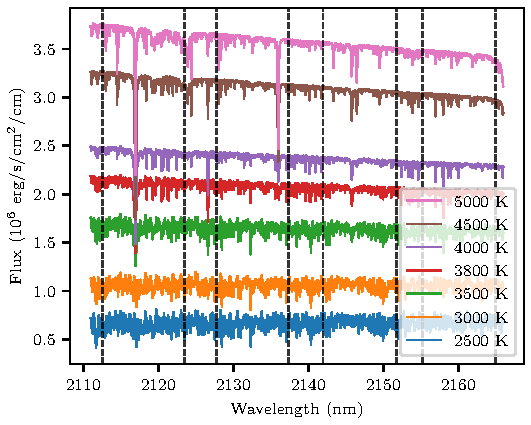
\includegraphics[width=\hsize]{./figures/companion_recovery/companion_spectra.pdf}
    \caption{{PHOENIX-ACES} spectra for temperatures between 2500 and 5000\K{}, corresponding to to the same lines in \cref{fig:injection_shape}.
The flux units are the native units of the {PHOENIX-ACES} spectrum, (\(\rm erg\,s^{-1}\,cm^{2}\,cm^{-1}\)), and have not been scaled by the stellar radii.
All spectra have a \logg{}=5.0 and \feh{}=0.0.
The vertical dotted lines indicate the edges of the CRIRES detectors.}
    \label{fig:comp_spectra}
\end{figure}

\subsubsection{Component {RV} separation}
\label{subsubsec:rv_seperation}
Another factor which could contribute to an unsuccessful detection is the {RV} separation between the host and companion, \Rvtwo{}.
Estimates for our observations are given in the last column of \cref{tab:observations}.
If \Rvtwo{} is small compared to the line width, then all the same lines of both components will be blended.
This is indeed the case for {HD~4747}, {HD~211847}, and {HD~202206} with expected \(|\rvtwo{}| < 2\)\kmps{}.
This may have contributed to the lack of recovery with both components of the binary model trying to fit to the same features.
This may even cause some correlation between the parameters of the two components.
The {RV} separation of the two components changes with orbital phase.
Having multiple spectra of the same target distributed in phase may allow the {RV} of the spectral components to be better recovered~\citep [e.g. ][]{czekala_disentangling_2017, sablowski_spectral_2016}.


\subsubsection {Wavelength range}
\label{subsubsec:wavelenght_range_limitation}
The wavelength choice for the spectra analysed here, observed with the intention to apply the spectral differential technique, was selected due to the location of the K-band telluric absorption window.
This wavelength range, with a narrow wavelength range \(\sim50\)\nm{} set by the CRIRES instrument.
This wavelength range is likely not the best choice for the proposed study.

Changing the wavelength coverage to regions with lines sensitive to stellar parameters for both stars and {BD}s, as well as using a larger wavelength range that will be achieved by CRIRES+, may help to improve the recovery results of the companion recovery technique presented here.
We note that if the wavelength range is increased by taking separate observations at different wavelengths, not covered by a single exposure, then changes in the {RV} of both components between the different wavelength observations may need to be accounted for.


\subsubsection{The {BT-Settl} models}
\label{subsubsec:bt-settl}
We note that the {PHOENIX-ACES} models are not the only spectral libraries available with the other notable library considered for this work is the {BT-Settl} models, ~\citep{allard_model_2010,allard_btsettl_2013,baraffe_new_2015}.
The included modelling of dust and cloud formation, as well as hydro-dynamical modelling atmospheric mixing/settling for atmospheres with \Teff{} below \(\sim2600\)\K{}, make the {BT-Settl} models valid across the regime from stars to {BD}s as cool as 400\K{}.
As the {BT-Settl} models are suitable to model the atmospheres of the brown dwarfs they would be useful for the companion recovery technique developed here.
However, as shown in \cref{subsection:results-hd211847, subsection:injection-recovery}, we were unable to successfully recover the 155\Mjup{} (\Teff{}\(\sim3200\)\K{}) low mass star companion of {HD~211847} and derived a temperature upper limit for our methodology of around 3800\K{}.
These are both well above the 2300\K{} cutoff of the {PHOENIX-ACES} models and for the onset of dust- and cloud-formation phenomena, at 2600\K{}.

\cref{fig:hd211847-models} shows again the minimum \textchisquared{} solution for detector 1 of the second {HD~211847} observation, this time including the {BT-Settl} solution with the same parameters.
Although the {PHOENIX-ACES} and {BT-Settl} models differ slightly they both have a large spectral mismatch to the observations.
As such, we did not use the {BT-Settl} models for the simulation and results above as we did not see any special advantage in using them.

The ease of access to find, download, and use {PHOENIX-ACES} spectral library, available in the fits file format, compared to older {BT-Settl} libraries is another reason for the current favoured use of the {PHOENIX-ACES} library.

Although the newer generations synthetic spectral models are improving and match the overall spectral energy distribution reasonably well there are still regions in the \emph{H}- and \emph{K}-band where there is room for improvement~\citet{rajpurohit_spectral_2016}.
The spectral mismatch in the region studied here is still too large for spectral recovery of companion brown dwarfs.
In the \nir{} we have compounding problem: the model input physics of sub-stellar temperatures and chemistry combined with the general difficulty of the \nir{}.

\begin{figure}
    \centering
    %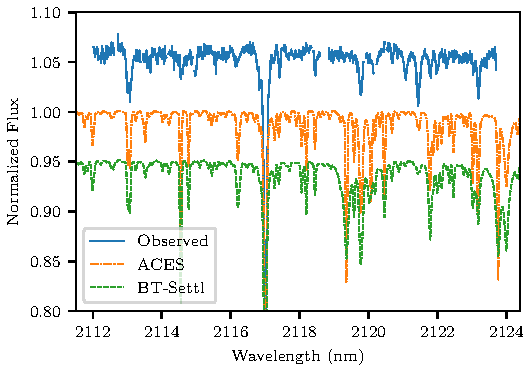
\includegraphics[width=\hsize]{images/final/HD211847_ACES_BTSettl.pdf}
    \caption{Detector 1 spectrum for {HD~211847} (blue) alongside the {PHOENIX-ACES} (orange dash-dot) and {BT-Settl} (green dashed) synthetic spectra for the host star only, with parameters \Teff{}=5700\K{}, \logg{}=4.5 and \feh{}=0.0.
        Both synthetic models have been normalized and convolved to \(\rm R=50\,000\).
        There is a 0.05 off-set between each spectrum}
    \label{fig:hd211847-models}
\end{figure}


\subsubsection{Impact of \logg{}}
\label{subsubsec:logg}
Logg, a measure of surface gravity, is related to evolutionary state and the size of the star with smaller \logg{} values usually indicating larger radii stars.
This parameter has a large impact on the radius and flux ratio of the binary models.
In the {PHOENIX-ACES} models a decrease in \logg{} from 5.0 to 4.5 increases the models effective radius by \(\sim\)1.75 in the temperature range investigated here.
This change in radius alone roughly triples (\(1.75^2\)) the absolute flux of the synthetic spectrum, neglecting any changes to the shape of the actual spectrum.
Therefore, there are large jumps in the model flux ratios if the \logg{} is allowed to vary, with lower \logg{} values for the companion being favoured as the increased flux ratio decreases the mismatch of the host component to the observations.
This large impact of \logg{} on the spectral library absolute flux is one reason for keeping the \logg{} of each component fixed in the \textchisquared{} results presented in \cref{sec:results}.

\subsubsection{Interpolation}
\label{subsubsec:interpolation}
It is common to interpolate between the synthetic spectral grids to fit and derive parameters in between the grid points~\citep[e.g.][]{nemravova_xtauri_2016, passegger_fundamental_2016}.
Instead of interpolation~\cite{czekala_constructing_2015} use a spectral emulator to use Principal Component Analysis to create eigenspectra for the synthetic library and Gaussian processes to derive a probability distribution function of possible interpolation spectra to account for uncertainties in the interpolation required for high signal-to-noise spectra.

However, we did not incorporate any interpolation into the companion recovery at this stage.
This could be something to be added in the future to refine the recovered parameters, and to help the transition between the grid \logg{} values.
Codes are readily available to perform spectral interpolation which could be utilized for this, two of them are \emph{pyterpol}\footnote{https://github.com/chrysante87/pyterpol}~\citet{nemravova_xtauri_2016} and \emph{Starfish}\footnote{https://github.com/iancze/Starfish}~\cite{czekala_constructing_2015}.


\subsection{Other techniques}
We note that there are many other disentangling techniques to separate mixed spectra of binary systems,~\citep[e.g.][]{hadrava_disentangling_2009}.
These require more than two observations, with  \(n+1\) observations used to set up a system of linear equations to solve for \(n\) spectral components~\citep[e.g.][]{simon_disentangling_1994,czekala_disentangling_2017, sablowski_spectral_2016}.
These methods are ideal for many well spaced observations.
For example the ideal situation for the {SVD} method of~\citet{sablowski_spectral_2016} is homogeneous samples of at least half the period, to identify the moving spectral components.
The few and insufficiently separated observations we analyse here are not suitable to apply any of these advanced techniques and are beyond what we have attempted here.










\subsection{Comparison to other methods}
kolbl 2014, passenger 2016, 2018

Contrast our result to other works.
More phases, longer integration time, higher {\snr{}}.



kobl 2015 also have difficult separating spectra with a {RV} separation below 10 km/s, or when the spectra of the spectra and companion have small separation.\todo{}


\textbf{
    CHECK out LOCKWOOD 2014 - maximum likelihood with todcor 1e-4 flux ratio double lined spectra}

